In this section our infrastructure is presented. The theory behind it is based on the horseshoe modernization model, which is depicts in Figure~\ref{fig:horseshoe}. As can be seen, this model consist of three steps, \textbf{Reverse Engineering}, (\textit{ii}) \textbf{Restructuring}, and \textbf{Forward Engineering}. The first step is represented by the left side of the horseshoe, it analyzes the legacy system in order to identify the components of the system and their interrelationships. Usually the reverse engineering step builds one or more representations of the legacy system at a higher level of abstraction (PSM). The second one is represented by the curve of the horseshoe since this steps takes the previous system's representation (PSM) and transforms it into another one (PIM) at the same abstraction level. Finally, the last step is represented by the right side of the horseshoe because it generates physical implementations (source-code) of the target system at a low abstraction level from the previously restructured representation of the system.

It worth noticing that KDM is the most essential part of our infrastructure. KDM supplies the representation and management of knowledge extracted by means of reverse engineering from all the different software artifacts of the legacy system. Therefore, the legacy knowledge obtained is then modernized into a target improved system by using the concept of MDD. As the infrastructure herein follows the three steps depicts in Figure~\ref{fig:horseshoe} then it has to go through five abstraction levels with four transformations among them. Both these abstract levels and the transformation are explained, as follows.

%Figure~\ref{fig:ADM_horse_shoe} depicts the horseshoe modernization model, the infrastructure is based in this model. This model consists of three steps, \textbf{Reverse Engineering}, (\textit{ii}) \textbf{Restructuring}, and \textbf{Forward Engineering}. The first step is represented by the left side of the horseshoe, it analyzes the legacy system in order to identify the components of the system and their interrelationships. Usually the reverse engineering step builds one or more representations of the legacy system at a higher level of abstraction (PSM). The second one is represented by the curve of the horseshoe since this steps takes the previous system's representation (PSM) and transforms it into another one (PIM) at the same abstraction level. Finally, the last step is represented by the right side of the horseshoe because it generates physical implementations (source-code) of the target system at a low abstraction level from the previously restructured representation of the system.

\begin{figure}[!h]
\centering
  % Requires \usepackage{graphicx}%left,bottom, right and top
 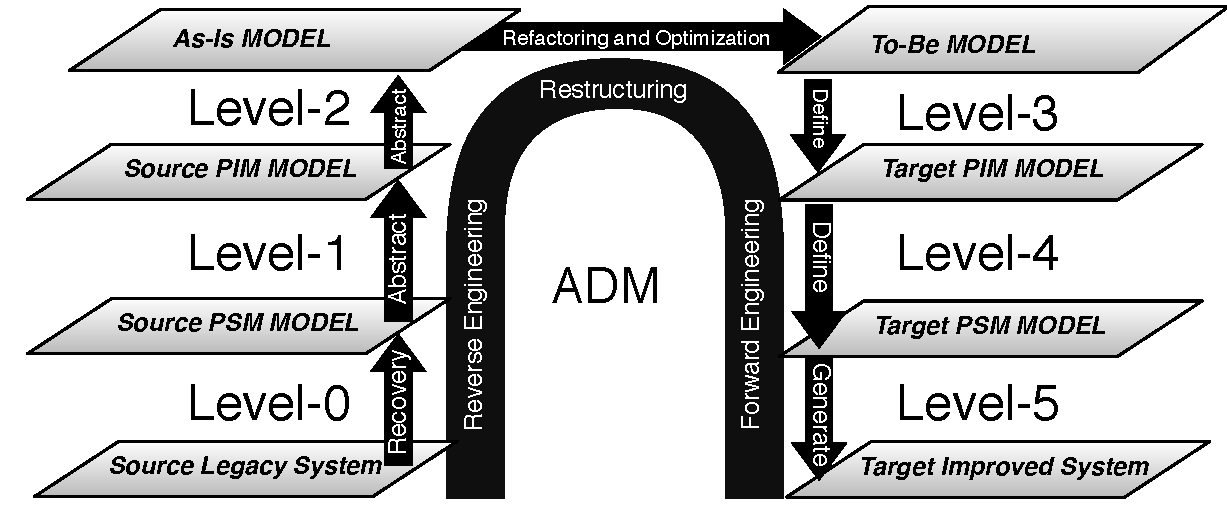
\includegraphics[%scale=0.063, clip=true, trim=32.23cm 18cm 5.45cm 13.853cm
 width=1\textwidth
 ]{Figuras/horseShoeBOM}
\caption{Horseshoe modernization model.}
\label{fig:horseshoe}
\end{figure}

In this section the Crosscutting Framework Integrated Reuse Environment (CrossFIRE) is presented. Figure~\ref{fig:proline} depicts a screenshot of CrossFIRE.

\begin{figure}[!h]
\centering
  % Requires \usepackage{graphicx}%left,bottom, right and top
 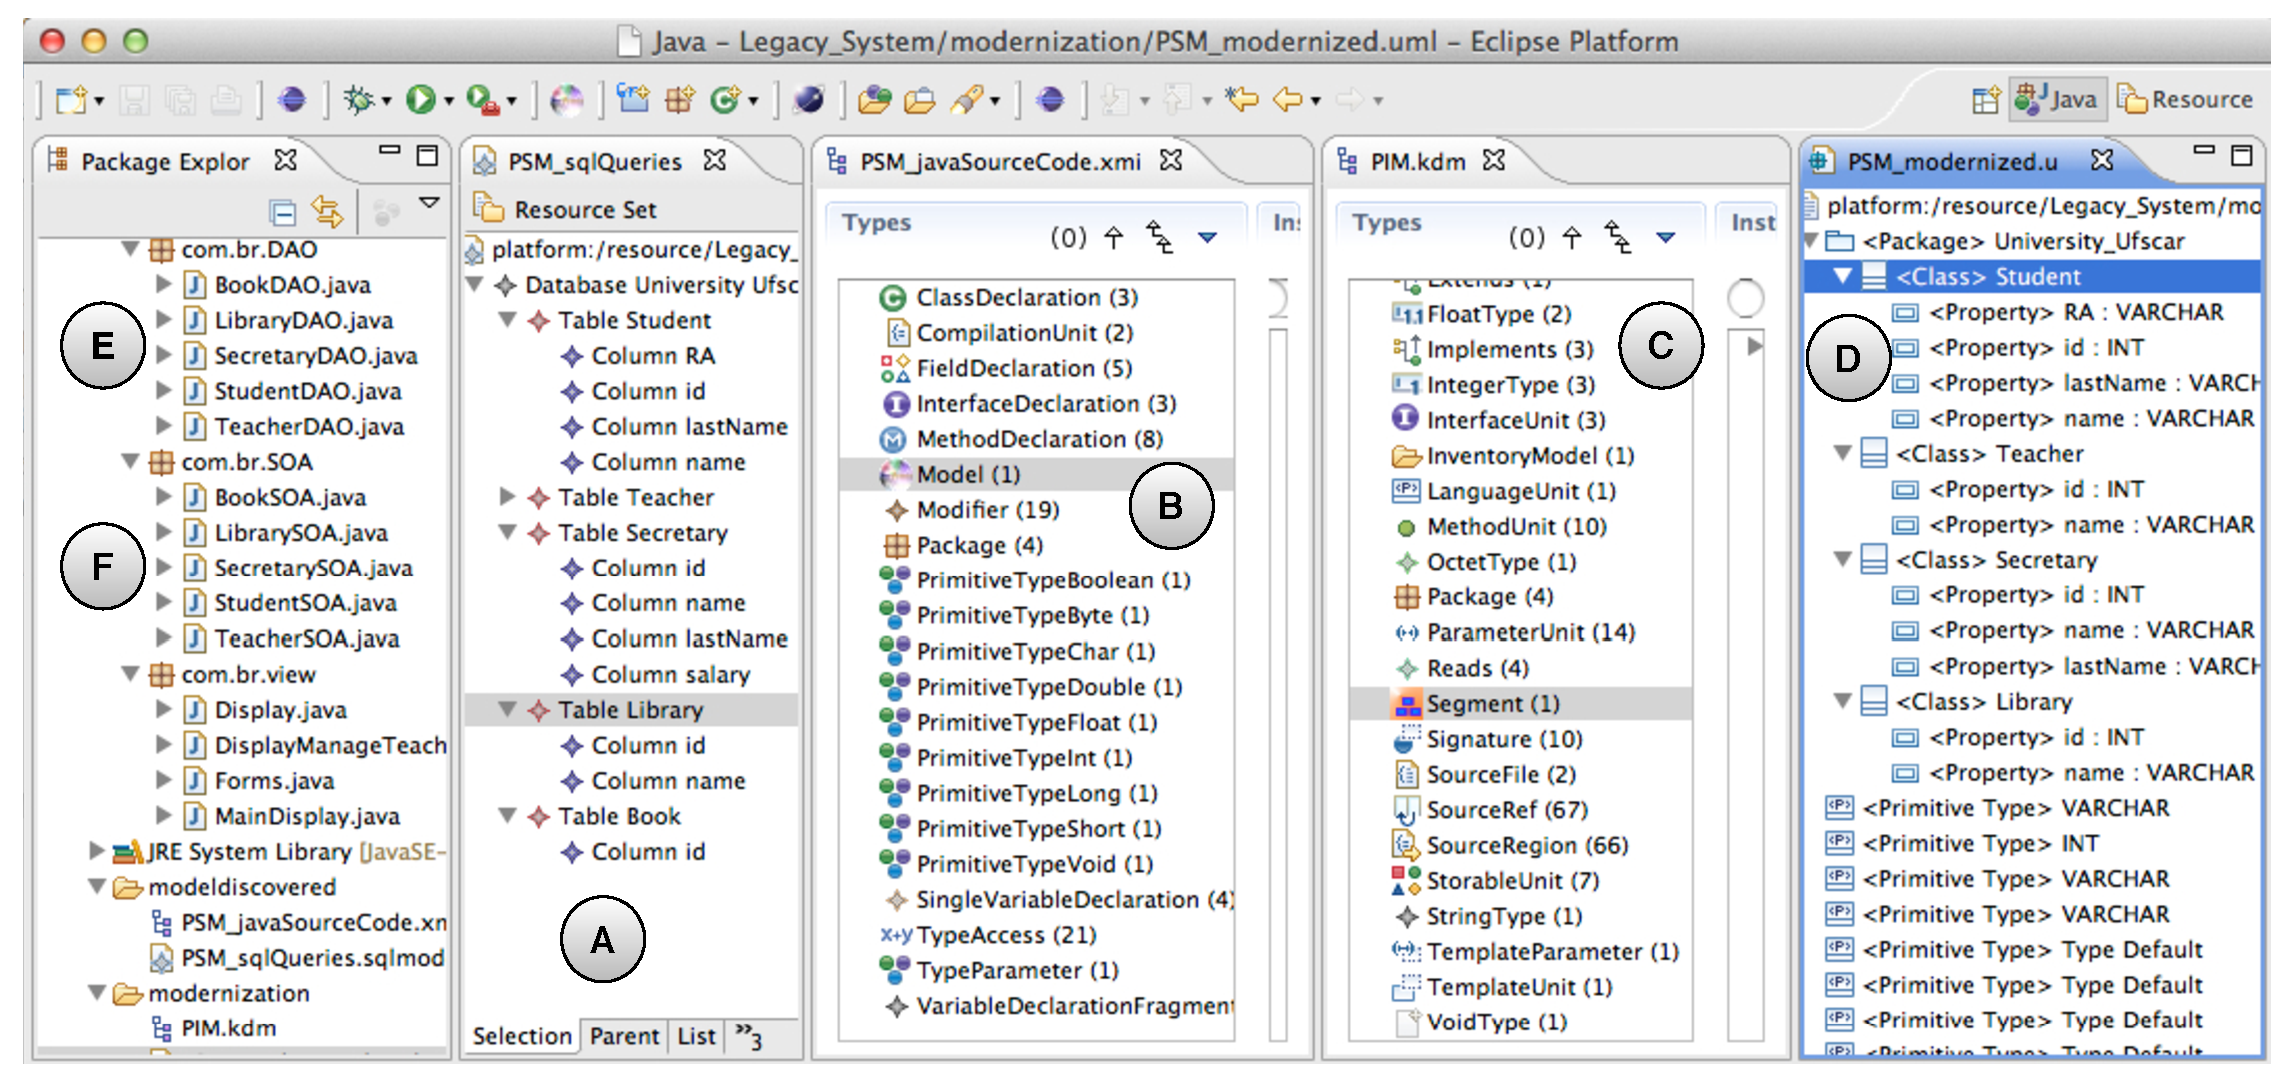
\includegraphics[%scale=0.063, clip=true, trim=32.23cm 18cm 5.45cm 13.853cm
 width=1\textwidth
 ]{Figuras/Tool}
\caption{Screenshot of CrossFIRE}
\label{fig:proline}
\end{figure}


All artifacts of the CF/CFF must be developed before one uses the CrossFIRE. Thus, it is worth highlighting that CrossFIRE only supports the Application Engineering (AE) phase. Having this in mind, the domain engineer has to use a traditional approach in order to create the artifacts in the Domain Engineering (DE) phase. In the DE phase, three artifacts must be created: (\textit{i}) source code of the whole CF, (\textit{ii}) the RRM and (\textit{iii}) the feature models of the CFF. These feature models have to be devised using the FeatureIDE\footnote{\url{http://wwwiti.cs.uni-magdeburg.de/iti_db/research/featureide/}}, which is a tool that provides a graphical way to assemble feature models. Afterwards, the engineer can use the CrossFIRE in order to uploaded these artifacts into a repository, as is shown in Figure~\ref{fig:proline}(A).    


In the AE phase, an application engineer can browse the repository in order to check whether there are CFs that can be reused in order to implement concerns of the planned application. In order to assist this activity, CrossFIRE provides a visualization, which depicts all CFs/CFFs that have been uploaded by the domain engineers.
Figure~\ref{fig:proline}(B) shows the visualization of all CFs/CFFs available.
As can be seen, there are six different CFFs - persistence, security, distribution, concurrency, logging and 	Business, respectively. 
In addition, CrossFIRE also shows descriptions for each of the selected CFFs by clicking on the button ``Description''. 
%Using this description the engineer can choose the CFFs. 
Nevertheless, if this description is not enough to help the engineer takes a decision on reusing the CF/CFF, CrossFIRE supplies a way to visualize the feature model related to selected CF/CFF by clicking on the button ``View'', Figure~\ref{fig:proline}(C). 
As is shown in Figure~\ref{fig:proline}(B), the ``persistence'' CF is highlighted to indicate that it has been chosen. 
Next, the ``Download'' button has to be clicked to transfer the feature model belonging to the CF chosen from the remote repository to the computer of the application engineer.

Furthermore, to reuse the CFF, its features must be chosen by the engineer aiming at specifying explicitly which features will be reused in the base application. %This is important because CFFs may have a great deal of features that probably will not be used in the application base. 
To assist this activity, CrossFIRE uses the ``configuration file'' of FeatureIDE. By using this ``configuration file'', features can be chosen by the application engineer. The graphical notation of the ``configuration file'' is shown in Figure~\ref{fig:proline}(D), which represents all features of the ``persistence'' CF. Moreover, FeatureIDE validates if the selected features match a valid combination for the instantiation of a member of the CFF. As shown in Figure~\ref{fig:proline}(D), once the application engineer has chosen the features (represented by ``+''), the resulting variant and constraints are generated automatically (represented by ``-''). 


The application engineer should provide  the selected features by using the ``configuration file'' to repository server, which will carry out an algorithm. This algorithm aims to extract two artifacts. The first extracted artifact only contains code related to the selected features. The second extracted artifact is a RM derived from a RRM, by removing unrelated requirements. The RM is used to support the reuse process of a CF. After that, these artifacts are sent to the application engineer's computer. %As can be seen in Figure~\ref{fig:proline}(3) the repository sent only the packages related to the features selected and specified through the ``configuration file'' i.e., the features Persistence, Connection and MySQL.


%he first artifact is the source code of the selected features

To reuse a member of the CFF or any other CF persisted in the repository, the application engineer may use the RM. It is graphically represented as a form which contains fields that should be filled with information regarding the base application. By completing this form, the code needed to couple the CF to the base application can be generated. It is possible to see our model editor in Figure~\ref{fig:rm}. 
The ``Palette'' on the right of the figure contains the elements of the RMs. They are:
 ``Group'': an element to group any element visible in the models;
 ``Pointcut'': represents join-points of the base application;
 ``TypeExtension'': represents types found in the base application;
 ``Value'': represents any numeric or textual values that must be informed while reusing the CF;
 ``Option'': defines a selectable variability of the framework and
 ``OptionGroup'': group selectable variabilities of the framework.

Each box contains a name and a description for the required information. The last line should be filled to provide the information regarding the base application. Note that the last line is only used  in RMs. For example, to be able to instantiate a persistence CF, the application engineer must specify methods from base application that should be executed after a database connection is opened and before it is closed.
Then, the box ``Connection Opening'' in  Figure~\ref{fig:rm} represents  names of methods that need an open database connection.
It is also needed to specify methods that represent data base transactions, and the variabilities must be chosen, e.g., the driver which should be used to connect to the database system. After filling the fields of the RM, a model transformation generates the code needed to couple the CF, and then, the reuse process is complete.
 Our tool also provides validation of the information filled into RM models.
 At the moment this paper was written, only AspectJ CFs are supported.

\begin{figure}[!h]
\centering
  % Requires \usepackage{graphicx}%left,bottom, right and top
 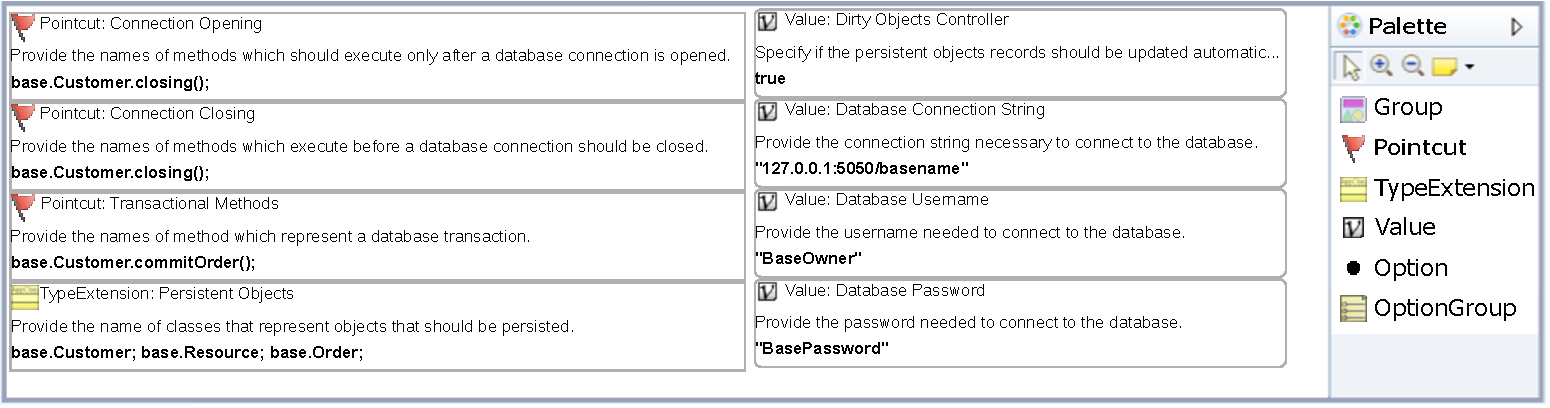
\includegraphics[%scale=0.063, clip=true, trim=32.23cm 18cm 5.45cm 13.853cm
 width=1\textwidth
 ]{Figuras/reuse_form}
\caption{Reuse Model Editor}
\label{fig:rm}
\end{figure}